\section{Auswertung}


\subsection{Vermessung der Nanostruktur}



\begin{figure}
  \centering
  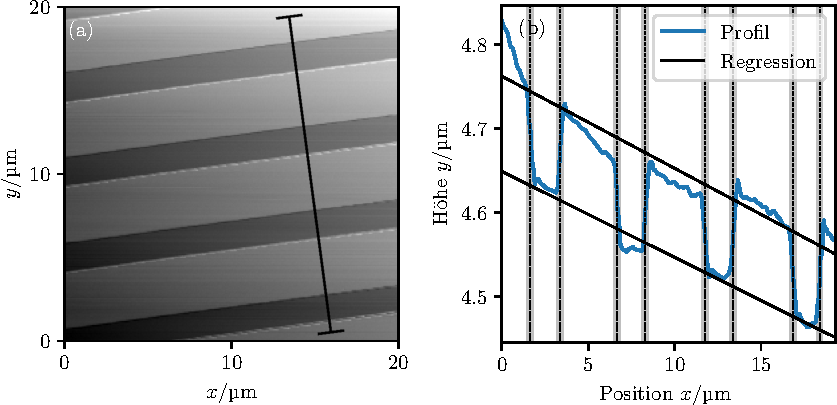
\includegraphics[scale = 1]{../analysis/data/nanostruktur_linien/linien_profil.pdf}
  \caption{Ergebnis der Messung an dem Linienprofil der Nanostruktur. (a) AFM Aufnahme mit eingezeichneten
  Linien, enlang derer das Profil in Abbildung (b) aufgenommen wurden. Das Profil ist
  über die Breite der in (a) eigezeichneten Balken gemittelt. Zudem sind in (b) die linearen Regressionen
  an die Datenpunkte eingezeichnet, die dem oberen bzw. unterem Niveau der Nanostruktur zugeordnet wurden.}
  \label{fig: linien_profil}
\end{figure}



\begin{figure}
  \centering
  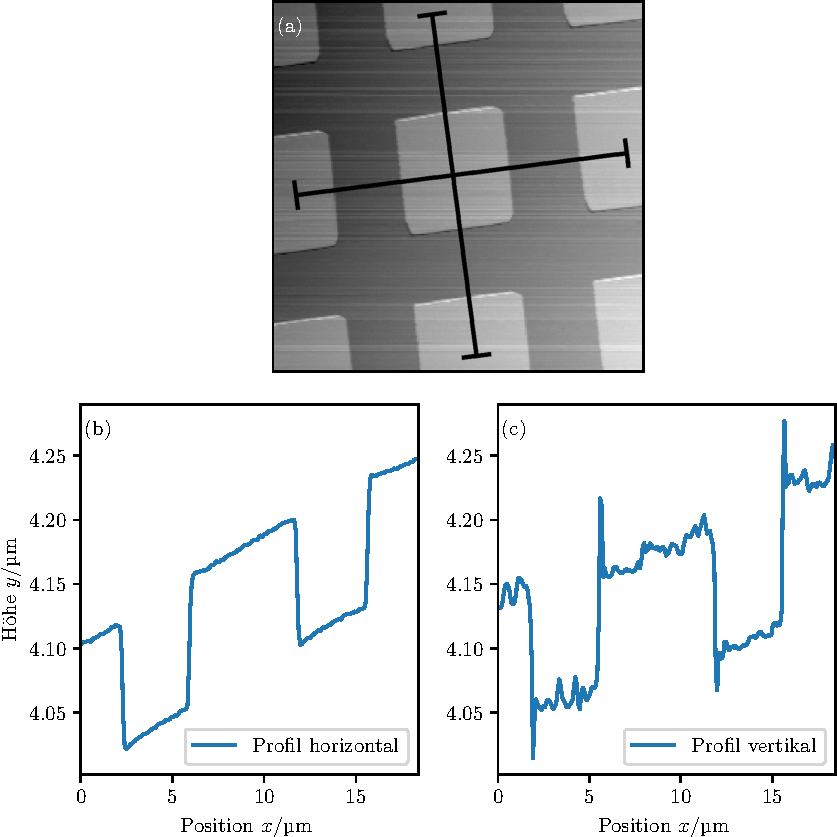
\includegraphics[scale = 1]{../analysis/data/nanostruktur_quadrate/quadrate_profile.pdf}
  \caption{Ergebnis der Messung an den quadratischen Nanostrukturen. (a) AFM Aufnahme mit eingezeichneten
  Linien, enlang derer die Profile in Abbildung (b) und (c) aufgenommen wurden. Die Profile sind
  über die Breite der in (a) eigezeichneten Balken gemittelt.}
  \label{fig: quadrate_profil}
\end{figure}



\begin{figure}
  \centering
  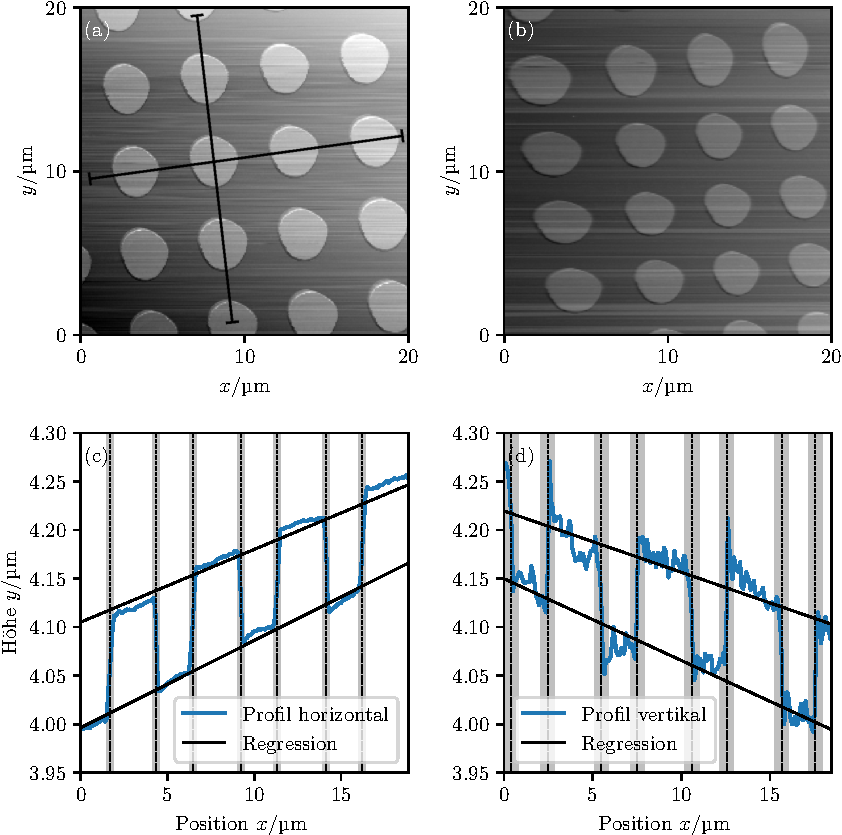
\includegraphics[scale = 1]{../analysis/data/nanostruktur_kreise/kreise_profile.pdf}
  \caption{}
  \label{fig: kreise_profil}
\end{figure}
